\chapter{Introduction}
%\epigraph{I remember a time when it was simple, it was just you and me; then there were three and in the midst of the chaos and dispair we became free.}

%\epigraph{In the beginning it was simple, it was just you and me; then there were three and in the midst of the turmoil we became free.}

%\epigraph{I remember a time when it was simple, it was just you and me; then there were three and in the midst of the turmoil we became free.}

\section{Background}
The $n$-body problem is a class of problems in physics that, in a highly general sense, consists of modelling the motion of $n$ objects interacting through some physical force. In classical mechanics the equations of motion for $n$ point particles can be derived from Newton's second law of motion, which states that the rate of change in momentum for an object equals the force acting on it, or from analytical formulations such as Lagrangian and Hamiltonian mechanics, which consider scalar properties of motion like kinetic and potential energies. In the non-relativistic quantum regime, where the wave-like property of matter has to be taken into account, the state of an $n$-body system is described by a total wave function, where the Hamiltonian operator generates the time evolution of the state as given by Schr{\"o}dinger's differential equation.

The core of the $n$-body problem is that neither the classical equations of motion nor the Schr{\"o}dinger equation are analytically solvable for more than two interacting particles. Consider the case where $n=3$. Although apparently simple, the configuration space for the three-body problem is six dimensional after separating out the centre of mass motion. Three additional constants of motion can be provided by conservation of the total angular momentum, which effectively reduces the problem to that of three coupled second order non-linear differential equations in the classical case and a three dimensional Schr{\"o}dinger equation in the quantum case. 

The quest for a general solution to the classical three-body problem is renowned. As a recurrent muse to a number of great mathematicians during the past centuries, dating back to Newton himself, the three-body problem has been a catalyst for the development of analysis and the modern theory of dynamical systems \cite{Chenciner2015}. Although there are a number of special cases that have explicit solutions, non-linear dynamical systems often display highly unpredictable behaviour due to sensitive dependencies on initial conditions, i.e., are chaotic. Nowadays, different numerical approaches are used to solve these kinds of problems, but the computational load can be substantial. 

In contrast to the classical case, the quantum three-body problem is amenable to qualitative analysis \cite{efimov1990qualitative} and, in some cases, even to analytic solutions. In the quantum realm of few-body systems the Faddeev and the Faddeev--Yakubovsky equations, which are equivalent formulations of the Schr{\"o}dinger equation for three- and four-body systems respectively, can, for a few special cases, be solved analytically by iteration \cite{Faddeev:1960su, Zubarev:1994}. For the three-body scattering problem bound state solutions can exist in cases where all three two-body subsystems have short-ranged interactions, if at least two of these interactions are close to resonance. This is called the Efimov effect. 

\section{The Birth of Efimov Physics}
In low energy scattering, particles are said to resonate when during the collision they remain close for an extended period of time, in an almost bound state, before separating. This kind of interaction is characterized by an $s$-wave scattering length that is much larger than the interaction range of the particles. 

In 1970, Vitaly Efimov predicted that resonant two-body forces could give rise to a series of bound energy levels in three-particle systems \cite{Efimov:1970zz}. When the short-ranged two-body forces approached resonance, he found a universal long-range three-body attraction emerging, giving rise to an infinite number of trimer states with binding energies obeying a discrete scaling law at resonance.  

Efimov proposed that attractive three-body interaction appearing in systems with resonant short-ranged interactions and repulsive Coulomb forces could explain the binding of three particle nuclei such as the three nucleon triton $\prescript{3}{}{\mathrm{H}}$ and the triple-alpha Hoyle state of $\prescript{12}{}{\mathrm{C}}$ \cite{Efimov:1970zz,Efimov:1971zz}.

The notion of Efimov physics comprises a range of universal phenomena that occur in few-body systems exhibiting the Efimov effect. Short-ranged forces commonly occur in nature and few-body effects are expected to appear in a broad range of physical systems. Development in the theory of few-body quantum systems is important, since it could bridge the gap between existing well developed models of treating one- and two-body systems and the statistical methods used to describe many-body systems.

\section{Theoretical Introduction}
A short review concerning some important aspects of quantum mechanical systems and two-body scattering, in particular the concept of \emph{scattering length}, will follow, in order to set the stage for a discussion of quantum effects in few-body systems in general and Efimov states in three-body systems in particular. A more detailed description of two-body scattering will be given in \Cref{chap:3}.

\subsection{Entering the Quantum Realm}
All particles of matter exhibit wave-like properties. The wavelength of a particle with momentum $p$ is given by the de Broglie equation

\begin{equation} \label{eq:1}
\lambda = \frac{h}{p} = \frac{h}{mv}
\end{equation}
where $h$ is the Planck constant. The wave characteristics of matter grow with increasing de Broglie wavelength. When the wavelength is sufficiently large, classical physics no longer applies and the system has reached the quantum regime. From \Cref{eq:1} it is evident that this is true for particles that are very small or very slow. In an ultracold quantum gas, the atoms are cooled down to a point where they move so slowly that the increased uncertainty in position for the individual atoms becomes so large that they start to overlap with each other. At this point the atoms can not be viewed as individual particles but as a correlated wave. The de Broglie wavelength of the atoms is then larger than the average interatomic spacing, which is typically about one micron in a low density gas, and their behaviour is fully governed by quantum mechanics. In other words, the transition to the quantum regime occurs when the thermal de Broglie wavelength is on the order of the interparticle spacing. Since the temperature of the gas and the thermal de Broglie wavelength are related through

\begin{equation}
\lambda_{\mathrm{th}} = \frac{h}{\sqrt{2\pi m k_{\mathrm{B}} T}},\label{eq:thermal}
\end{equation}
in which $k_{\mathrm{B}}$ is the Boltzmann constant, it means that there is a critical temperature for when the quantum effects become dominant.\footnote{In an ideal gas, the thermal de Broglie wavelength $\lambda_{\mathrm{th}}$ is the average de Broglie wavelength of the gas particles at the specified temperature. Since the average interparticle spacing is approximately given by $(V/N)^{1/3}$, where $V$ is the volume and $N$ is the number of particles, the quantum effects will dominate for temperatures where $(V/N)^{1/3} \leq \lambda_{\mathrm{th}}$, while the gas will behave classically for temperatures where $(V/N)^{1/3} \gg \lambda_{\mathrm{th}}$. Transitions between these two regimes in a gas of free particles with masses $m$ occur at a critical temperature $T=T_{\mathrm{c}}$ when $(V/N)^{1/3} \sim \lambda_{\mathrm{th}}$. This transition temperature is inversely proportional to the particle mass, see \Cref{eq:thermal}.} For a dilute atomic gas this critical temperature is in the microkelvin to nanokelvin range.

\subsection{Two-body Interactions}
Atomic interactions are, to a good approximation, pair-wise and short-ranged, which means that they interact when they are close to each other. At sufficiently low energies, atoms behave like point particles and have quantized orbital angular momenta $l$. In analogy with atomic orbitals, the quantum numbers $l=0,1,2,$ associated with an atom, are referred to as $s$-waves, $p$-waves and $d$-waves, respectively. 

After separating out the centre-of-mass, the scattering processes of two particles can be expressed in terms of their relative position only. The relative motion can be decomposed into that of an incoming plane wave, expanded into a sum of partial waves with definite angular momenta, which scatters off a potential placed at the origin. For low energy scattering, only the first few $l$-quantum numbers contribute to the scattering process and in the ultracold regime $s$-wave collisions dominate. Scattering becomes isotropic when the wavelength of the relative motion is much larger than the typical interparticle interaction range $r_0$, since the wave is then too large to resolve the details of the short-range interaction. In other words, the colliding atoms cannot resolve each other's internal structure given by their electron configurations. This makes scattering in the low energy limit indistinguishable from that of point particles provided that the mean distance between the atoms is much larger than the interaction range, which is the case in a low density atomic vapour. Furthermore, only spherical waves will come close enough to be scattered by the potential. Higher partial waves ($l>0$) will not ``feel'' the potential since they will be reflected by a centrifugal barrier at separations greater than the interaction range. Two-body scattering in this regime is solely governed by a single parameter called the $s$-wave scattering length $a$. The $s$-wave scattering length, referred to as `the scattering length' from here on, is defined in the low-energy limit as

\begin{equation} \label{eq:2}
a = \lim_{k \to 0} -\frac{\tan\delta_0(k)}{k},
\end{equation}
where $k$ is the wave number ($k=p/\hbar = \sqrt{2\mu_{2\mathrm{b}} E}/\hbar$), $E$ is the kinetic energy of the relative motion, $\mu_{2\mathrm{b}}$ is the two-body reduced mass and $\delta_0(k)$ is the $s$-wave phase shift of the outgoing wave. For small $k$, the phase shift will behave as $\delta(k)\approx-ka + O(k^2)$. If scattering by a hard sphere is considered, the scattering length $a$ is simply the radius of the sphere. In the low energy limit, the scattering properties for an arbitrary potential with positive scattering length is the same as that of a hard sphere with radius a. Alkali atoms, however, often have a scattering length with a magnitude that is much larger than the interaction range.\footnote{For large atomic separations the van der Waals interaction, which is caused by electric dipole--dipole interactions between the atoms, is attractive and of the form $-C_6/r^6$. In low-energy scattering of alkali atoms this potential dominates the interactions between a pair of particles. The large scattering lengths of alkali atoms, which are typically about two orders of magnitude greater than the Bohr radius $a_0$, are due to the particularly large values of the van der Waals coefficients $C_6$ for the ground state atoms in this group. 
	
The basic scale of the scattering length is set by the length scale $l_{\mathrm{vdW}}$ in the zero-energy Schr{\"o}dinger equation, which can be estimated using dimensional arguments for the order of the kinetic and the potential energy and then equating these two at $r \sim l_{\mathrm{vdW}}$  \cite{pethick_smith_2008}. With the kinetic energy $ \sim \hbar^2/2\mu_{2\mathrm{b}}l_{\mathrm{vdW}}^2$ and the potential energy $ \sim C_6/l_{\mathrm{vdW}}^6$ this length scale, which is often referred to as `the van der Waals length' or `the characteristic range of interaction', is then given by $l_{\mathrm{vdW}} \approx (2\mu_{2\mathrm{b}} C_6/\hbar^2)^{1/4}$ \cite{BRAATEN2006}. However, even though the basic scale of the scattering length is set by $l_{\mathrm{vdW}}$, the sign and numerical value of $a$ is determined by the details of the short-range interaction and there are several examples among the alkali atoms where the two-body interaction is accidentally fine-tuned in a way that yields a scattering length that is unnaturally large, i.e., $\abs{a} \gg l_{vdW}$. More importantly, these atoms have interactions that can be tuned artificially, which means that $a$ can be set to an arbitrarily large value.

In the field of Efimov physics it is common to define the van der Waals length as $r_{vdW}=l_{\mathrm{vdW}}/2$ and for that reason this is the definition that will be used later on in this work.} 
Scattering can therefore occur at separations greater than the interaction range if the magnitude of the scattering length is sufficiently large. Consequently, at large separations the scattering length characterizes the effective interparticle interaction when the energy is very low. Since a positive scattering length corresponds to a negative phase shift, i.e., to the scattered wave being pushed out, the effective interaction will be repulsive (\Cref{fig:phaseshift_a}). Conversely, a weakly attractive potential will pull in the wave function, corresponding to a negative scattering length and an effective attractive interaction (\Cref{fig:phaseshift_b}). However, as I will discuss below, this simple picture becomes more complex if the attractive potential is deep enough to support a bound state. For an attractive potential that cannot support a bound state the scattering length is negative and the effective interaction at large separations is attractive. On the other hand, if the potential can support one, or more, bound states, it is possible to have both positive and negative scattering lengths, thus corresponding to both effective repulsive and effective attractive interactions. If the depth of the underlying attractive two-body potential is increased when $a$ is positive, $a$ will decrease and the outward push of the wave will lessen as the effective repulsion decreases. If the potential is made more attractive when the scattering length is negative, however, the effective interaction will become more attractive, since the increased positive phase shift will cause the scattered wave to be pulled in further. 

\begin{figure}[h!]
	\centering
	\subcaptionbox{The wave function is pushed outwards when the magnitude of a positive scattering length is increased.\label{fig:phaseshift_a}}{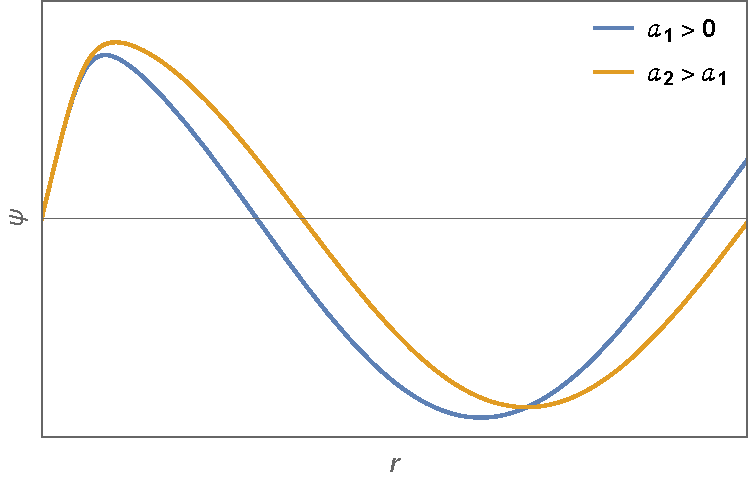
\includegraphics[width=0.47\textwidth]{pos_scat.pdf}}
	\hfill % <-- Seperation
	\subcaptionbox{The wave is pulled inwards when the magnitude of a negative scattering length is increased.\label{fig:phaseshift_b}}{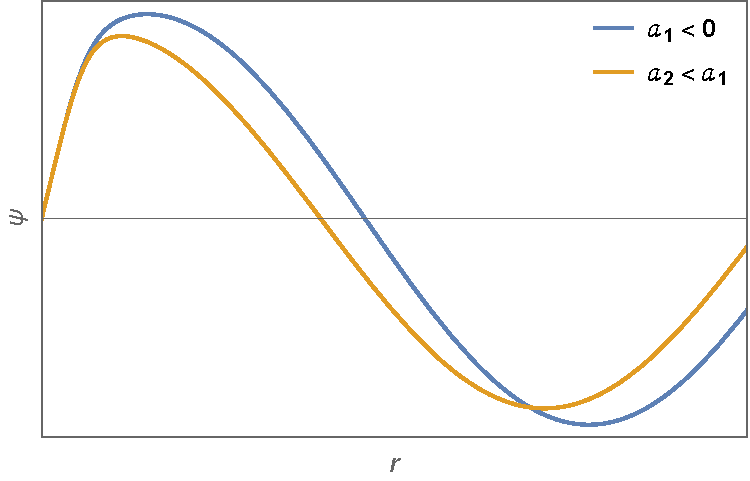
\includegraphics[width=0.47\textwidth]{neg_scat.pdf}}%
	\caption{Illustration of phase shifts causing an effective interaction and how they depend on the sign and magnitude of $a$.}\label{fig:phaseshift}
\end{figure}

In the absence of an interaction, the phase shift is simply zero and the outgoing scattered wave is in phase with the incoming wave. Any interaction will cause a dephasing between the outgoing and incoming waves. The larger the dephasing is, the larger the effect of the scattering potential on the asymptotic wave will be. The strongest dephasing occurs when $\delta_0$ takes the value $\pi/2 \pmod{\pi}$, whereupon two-body $s$-wave resonances are formed and the scattering length, as defined in \Cref{eq:2}, diverges. At this point a node appears in the inner part of the wavefunction. If the potential depth is increased further, the scattering length becomes $\pm \infty$ and then again decreases until the appearance of another bound state, where it once again diverges. This behaviour is illustrated in \Cref{fig:res_1}. The situation when the scattering length diverges is of particular interest in this thesis because Efimov physics arises when the two-body interactions are near resonance. Since the phase shift for the $s$-wave can be written as $\delta_0 \propto -ka$ in the long wavelength limit ($k \ll r_0^{-1}$), it means that the scattering length $a$ has to become much larger in magnitude than the interaction range $r_0$ for a two-body interaction to become resonant.

\subsection{Universality}\label{sec:universality}
Particles with large scattering lengths, i.e., $\abs{a}\gg r_0$, in the low-energy regime, have universal properties. The properties are universal in the sense that they depend on the scattering length alone and not on the details of the short-range interaction. Alkali atoms interact via van der Waals potentials of the form $-C_6/r^6$, where the range $r_0$ typically is on the order of the van der Waals length, which can be defined by \cite{vanderWaals}

\begin{equation}
r_{\mathrm{vdW}} = \frac{1}{2}\bigg(\frac{2\mu_{2\mathrm{b}} C_6}{\hbar^2}\bigg)^{1/4}.
\end{equation}

For a system of two identical bosons with $a>0$ there is a universal shallow two-body bound state near the scattering threshold, with the binding energy 
\begin{equation}\label{shallowdimer}
E_D = \frac{\hbar^2}{ma^2}.
\end{equation}
For $a<0$ there is no such bound state. Outside the universal range the natural binding energy for two particles should be approximately $\hbar^2/mr_0^2$. The cross section for elastic scattering of two identical bosons in this regime is also universal and so is the mean square radius of the bound molecular state, which are given by

\begin{equation}\label{elasticcross}
\sigma = 8\pi a^2
\end{equation}
and

\begin{equation}\label{meanradius}
\langle r^2\rangle = \frac{a^2}{2},
\end{equation}
respectively, in zero energy limit. The universal quantities given in \crefrange{shallowdimer}{meanradius} are exact for $a=\pm \infty$ and approximate for $\abs{a}\gg r_0$. The unique dependence on this one length parameter also leads to continuous scaling symmetries in these quantities. If the scattering length is scaled with some real factor $\lambda$ such that $a \to \lambda a$, the shallow dimer energy will scale as 

\begin{equation}
E_D(\lambda a) = \lambda^{-2}E_D(a),
\end{equation}    
while the elastic cross section and the mean square radius scale as 

\begin{equation}
\sigma_e(\lambda^{-1}k,\lambda a) = \lambda^2 \sigma_e(k,a)
\end{equation}
and

\begin{equation}
\langle r^2(\lambda a)\rangle = \lambda^2 \langle r^2(a)\rangle ,
\end{equation}
respectively. 

While the scattering length completely governs the low energy two-body collision problem, it is also the main parameter for describing the interaction of particles at very low collision energies in general. 

Similarly to the universal quantities found in the two-body sector, three-body systems can also exhibit universal properties. For particles interacting through short-ranged interactions near resonance, i.e., when the attraction is on the verge on or just barely can support a shallow dimer, corresponding to $\abs{a}=\infty$, an effective long-range three-body attraction emerges, which can form shallow three-body bound states.

To understand how this long-range interaction is formed, consider a collision between the shallow dimer and a third particle in the low energy limit. The third particle will start to ``feel" the dimer at a distance close to the magnitude of the two-body scattering length, which is also the size of the dimer. At this point the third particle could tug off any of the particles in the dimer to form a new pair. By flickering back and forth between the two particles, the third particle can mediate an interaction between the two, and even when the interaction is not strong enough to support any bound binary subsystem, it may still support one or more trimer states.\footnote{The binding of three particles, while all three two-body subsystems are unbound, is called Borromean binding. As the name implies, the state falls apart into three free particles if one particle is removed. Similarly to the linking of the Borromean rings, stability of the state is secured by the three when no bound pairs can form \cite{Kajsa_my}.} It is this process of particle exchange that results in the effective three-body interaction that Vitaly Efimov found when he was studying the quantum three-body problem. This effective long-range attraction is universal in the sense that it emerges irrespective of the underlying two-body short-range interactions and, in the resonant limit, it gives rise to an infinite series of bound states, called Efimov trimers.

Two aspects of universality in the three-body sector for three identical bosons are that the size and energy of successive trimer states in the resonant limit are related by a scale transformation with a constant $\lambda = e^{\pi/s_0} \approx 22.7$, where $s_0 \approx 1.00624$ is a universal constant of Efimov physics. The continuous scale invariance, which appears in the two-body sector, is therefore not applicable. Instead, the symmetry of the asymptotic Efimov spectrum is characterized by a discrete scale invariance where the size and binding energies each form a geometric progression, where the size of an excited state is larger than the previous state by the factor $\lambda$ and the binding energies of two consecutive states scale like $E_T^{n+1} = E_T^{n}\lambda^{-2}$.   

The Efimov scenario is illustrated in \Cref{fig:efimov} where the energies of the three lowest trimers are plotted as functions of $1/a$. Three different regions can be identified in the figure. The region above the zero-energy threshold is the three atom continuum. In grey is the trimer region, where the bound Efimov states are shown schematically by solid blue lines (with a scaling factor set at $1.7$ rather than $22.7$ for illustrative purposes). On the positive side of $1/a$ the Efimov trimer states merge into the atom-dimer continuum.

\begin{figure}
	\centering
	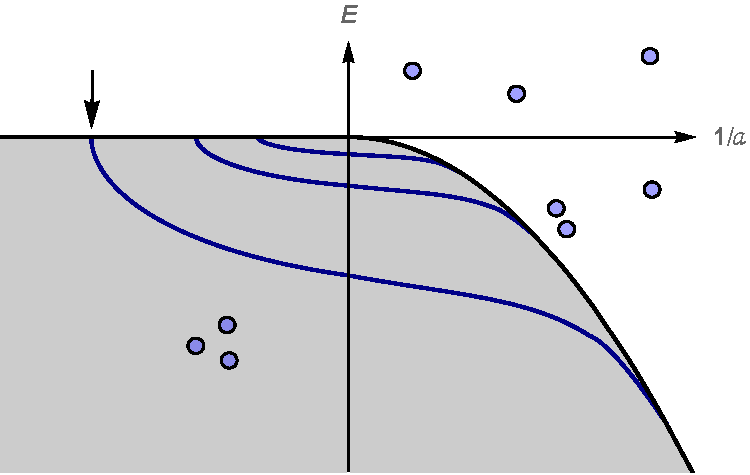
\includegraphics[width=0.75\linewidth]{efimov_spec_a}
	\caption{The energies of the three first Efimov states are plotted as functions of the inverse scattering length $a$. Three different regions can be identified in the figure: The three atom continuum is the region above the zero-energy threshold; the atom-dimer region is the region enclosed by the horisontal axis and the atom-dimer threshold (the solid black line); and the trimer region is the region shown in grey, where the Efimov states are represented by the blue lines. The value $1/a_-^{(0)}$ for where the first Efimov resonance appears is marked by an arrow.}\label{fig:efimov}
\end{figure} 

Universality in the three-body sector is different from that in the two-body sector in the way that it requires an additional parameter, which incorporates all relevant short-range interactions among the three particles that are not included in the two-body scattering length. The three-body parameter can be defined as the value of the scattering length $a_-^{(0)}$ at which the first Efimov resonance appears in the spectrum (the value $1/a_-^{(0)}$ is marked by an arrow in \Cref{fig:efimov}). The three-body parameter fixates the location of the Efimov ground state and, together with the universal scaling constant, therefore determines the entire energy spectrum of three identical bosons, since the position of the coupling to the three atom continuum for each consequtive resonant state is given by the geometric sequence $a_-^{(n)}=a_-^{(0)}\lambda^n$. However, the value of $a_-^{(0)}$ was expected to be non-universal since it depends on the details of the short-range molecular interaction via a three-body phase shift. As it turned out, this was not case and I will return to that in \Cref{chap:2}.

The Efimov effect is not limited to systems of identical bosons and can, in fact, appear in a variety of systems, such as in systems of bosonic unequal masses and in three component Fermi-Fermi mixtures. However, the universal scaling constant will then assume a different value since it is system dependent in the sense that it depends on the statistics of the particles involved, i.e., whether they are fermions or bosons, and their mass ratio. 

\section{Thesis Objective}
The main purpose of this thesis is to summarize the theory of Efimov physics and the methodology used for developing a computer code that calculates the effective long-range three-body potentials, which later can be used to calculate the Efimov energy spectrum and three-body wave functions. 

\section{Outline}
The thesis is organized as follows: \Cref{chap:2} serves as an introduction to the reader of some of the main experimental findings in the field of Efimov physics; a brief review of the theory of quantum mechanical scattering is given in \Cref{chap:3} with a focus on low energy and zero energy scattering; in \Cref{chap:4} I present the theory of the three-body scattering problem and introduce both non-symmetric and symmetric hyperspherical coordinates; \Cref{chapter:5} outlines the numerical method used to develop the computer code; in \Cref{chapter:scattering_model} I describe the scattering model used to test the validity of the code; in \Cref{chap:7} I present and analyze the results; and in \Cref{chap:8} I conclude the work and propose an idea for future studies.
